%\documentclass[11pt]{book}
%
%\setlength{\parindent}{0pt}
%\setlength{\parskip}{8pt}
%
%\usepackage{amsmath}
%\usepackage{amssymb}
%\usepackage{hyperref}
%\usepackage{cleveref}
%
%\renewcommand*{\thefootnote}{\fnsymbol{footnote}}
%
%\setcounter{chapter}{3}
%
%\begin{document}
%
%\section*{A Levelized Comparison of \\ Pulsed and Steady-State Tokamaks}
%
%\let\cleardoublepage\relax \tableofcontents \newpage

\chapter{Planning Future Work \added{for the Model}}

\added{This model may run and produce interesting results, but there is always more to be done. This chapter explores three potential fusion reactors that could help guide real world designs. These are: a stellarator (Ladon), a steady-state/pulsed \replaced{composite}{hybrid} (Janus), and a tokamak capable of reaching H, L, and I modes (Daedalus). The chapter then concludes by describing several possible model improvements, including: adding radiation sources, using pedestal profiles, and improving flux balance.}

\deleted{This model may run and produce interesting results, but there is always more to do. This chapter explores three potential fusion reactors that could help guide real world designs. It then goes into a laundry list of possible model improvements.}

\deleted{The three reactors covered are: a stellarator (Ladon), a steady-state/pulsed hybrid (Janus), and a tokamak capable of reaching H, L, and I modes (Daedalus).}

\section{Incorporating Stellarator Technology -- Ladon}

A stellarator is, at a basic level, a tokamak helically twisted along the length of its major circle. For a long time they were dismissed because of \replaced{their poor transport properties.}{the difficulty involved in building spiraled magnets.}  Recent technological improvements, though, have eased this situation -- as seen with the Wendelstein 7-X device in Germany. The problem now is engrained in the \replaced{underdeveloped}{missing} scaling laws stemming from a lack of machines and, more fundamentally, data points.

\begin{figure}
	\centering
	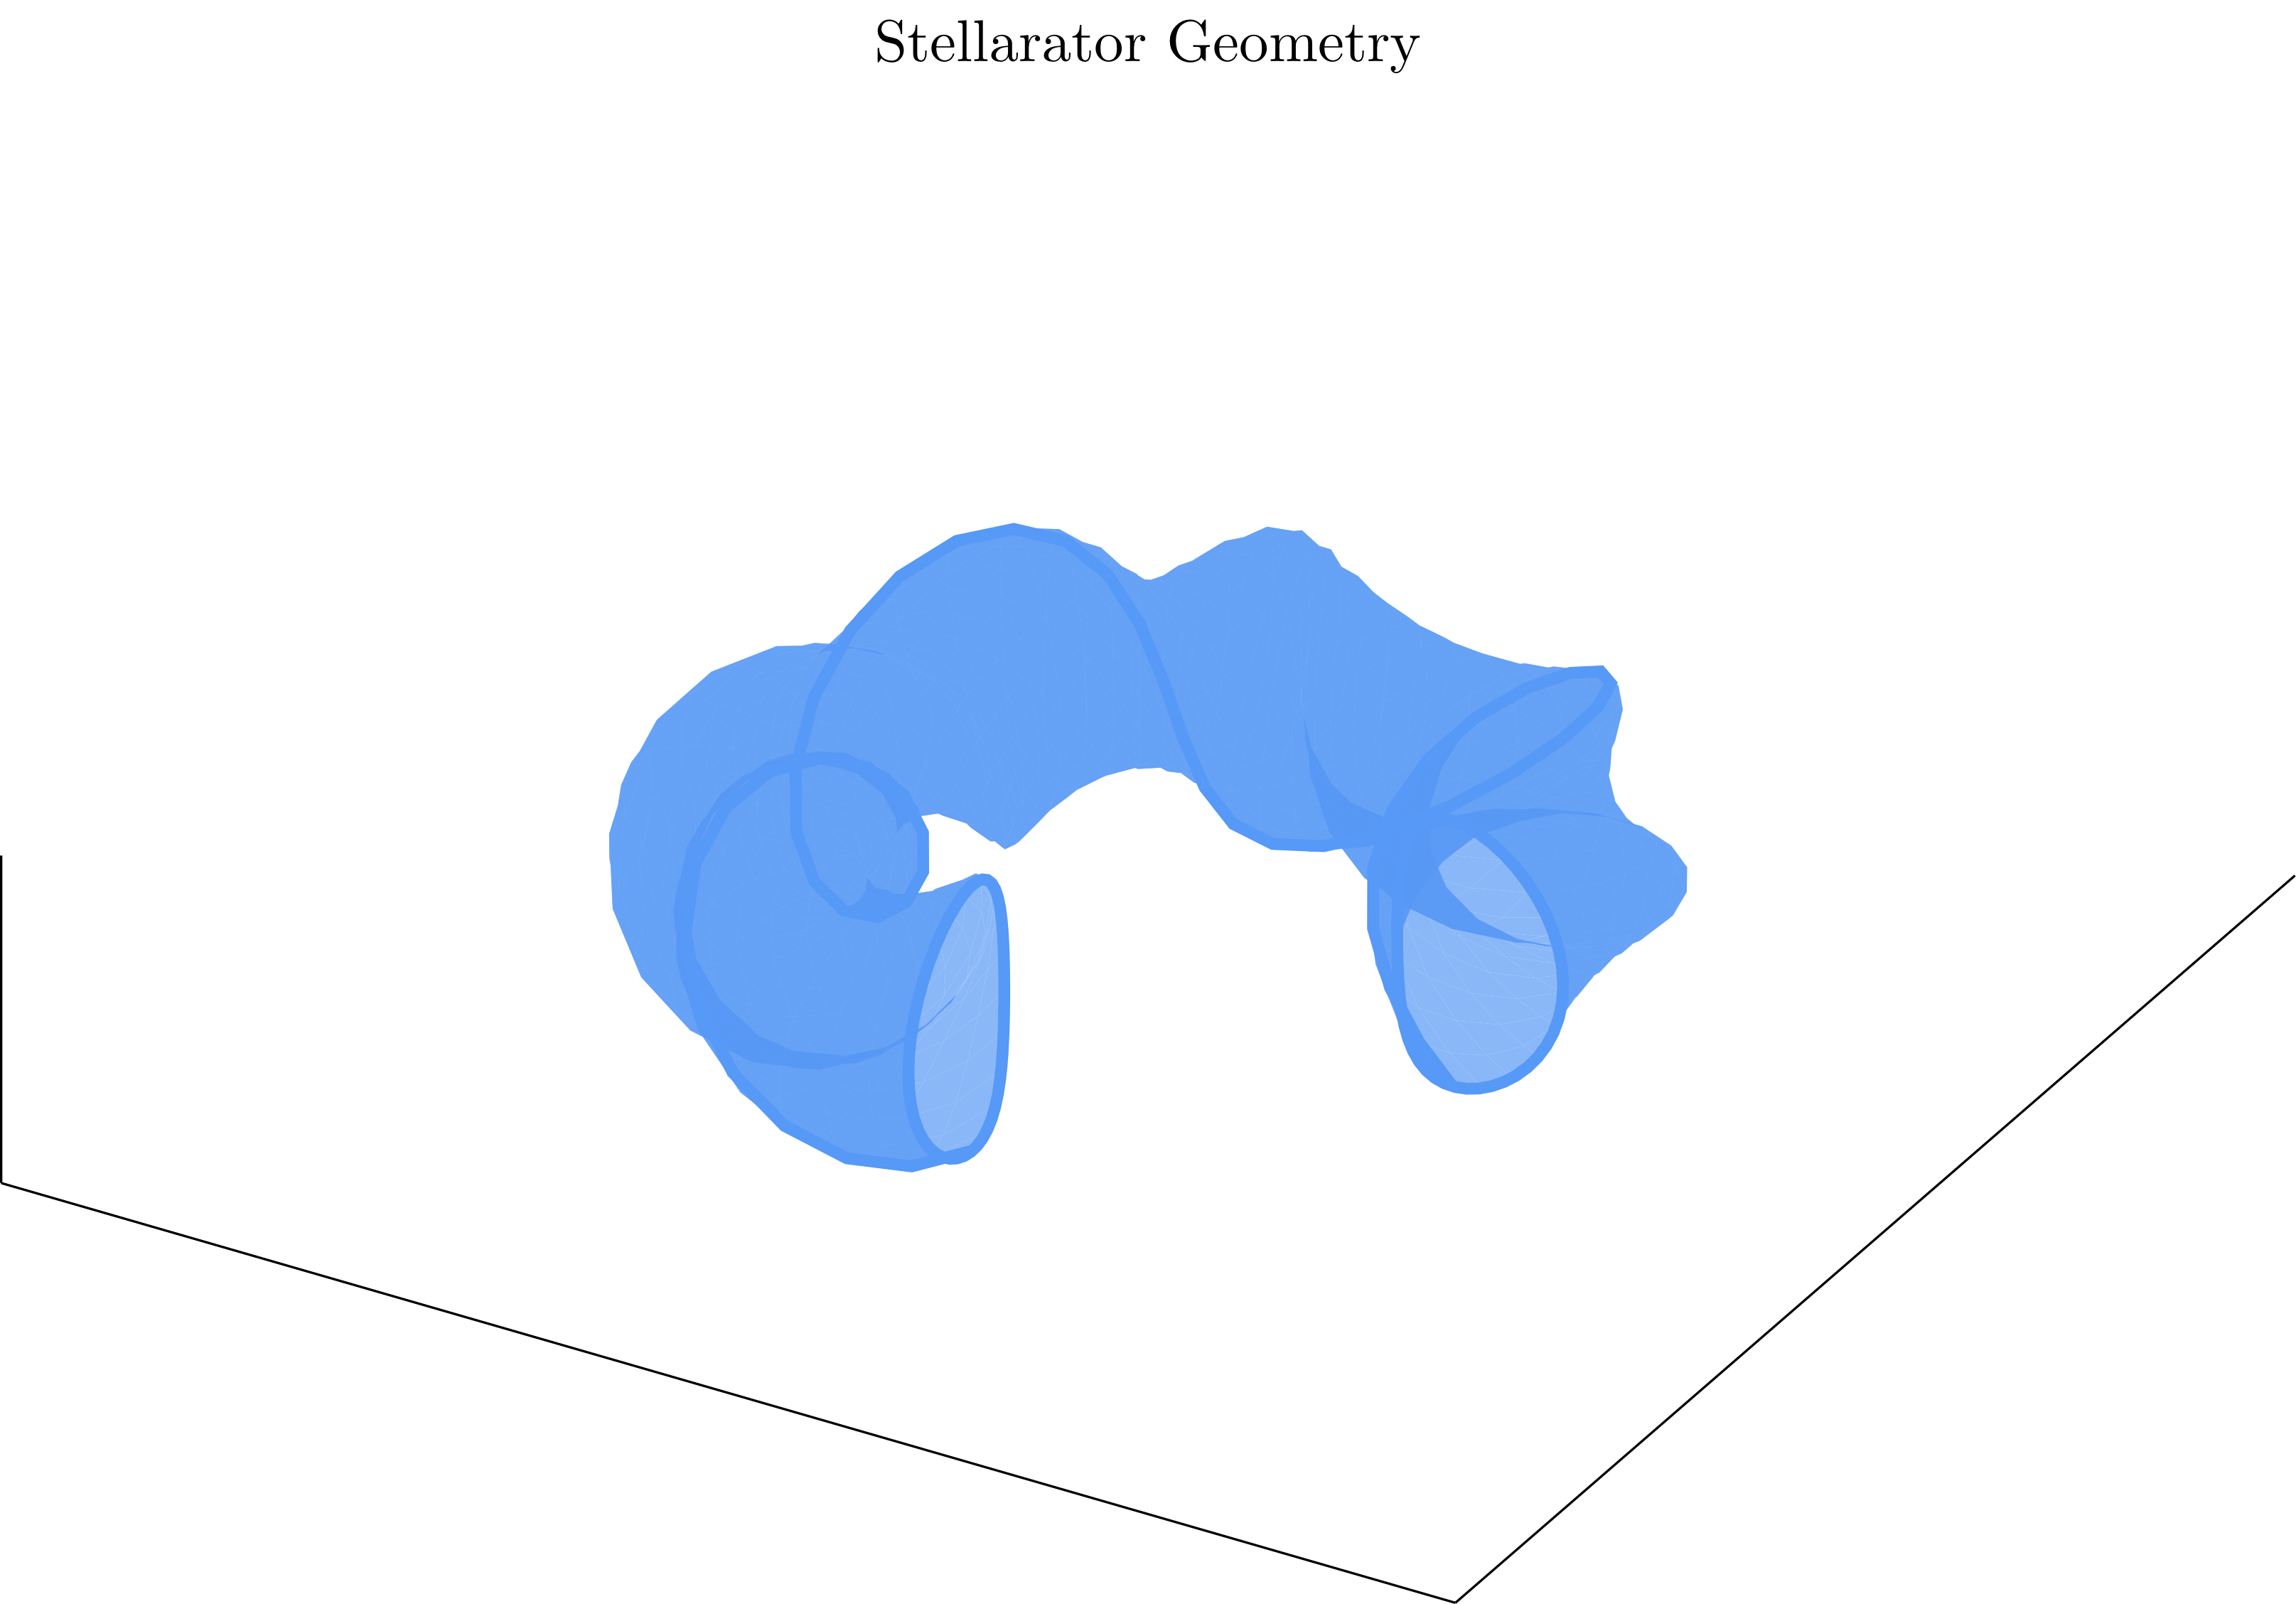
\includegraphics[width=0.75\textwidth]{images/stellarator}
	\caption{Cut-Away of Stellarator Reactor} ~\\
\end{figure}

\added{To model Ladon, this paper's proposed stellarator, one would need to replace at least: the Greenwald density limit and the confinement time scaling law. In place of the Greenwald density will likely be some other density or current limit, possibly the Bremsstrahlung density limit.\cite{stellar} This may require the density to be carried throughout analysis -- thus appearing explicitly in one column of \cref{table:eq}.}

\deleted{Optimistically, expanding this model would just involve developing a new confinement time scaling law and replacing the Greenwald density limit. The reason the Greenwald density limit is no longer important is because stability is much easier to maintain in a stellarator. Most likely, the density limit will now be governed by Bremsstrahlung radiation. If this were the case, each equation would need to be redivided using it. Ladon would be the reactor built using this enhancement.}

\section{Making a \replaced{Composite}{Hybrid} Reactor -- Janus}

The next interesting reactor would be a \replaced{composite}{hybrid} tokamak incorporating pulsed and steady-state operation: Janus. Fundamentally, this would involve current coming from both LHCD (steady-state), as well as inductive (pulsed) sources. This was actually used in Demo Pulsed, but the current drive was not handled self-consistently. Coupling these two current sources could reduce reliance on bootstrap current and lead to much more compact machines.

\begin{figure}
	\centering
	\begin{adjustbox}{width=0.75\textwidth}
		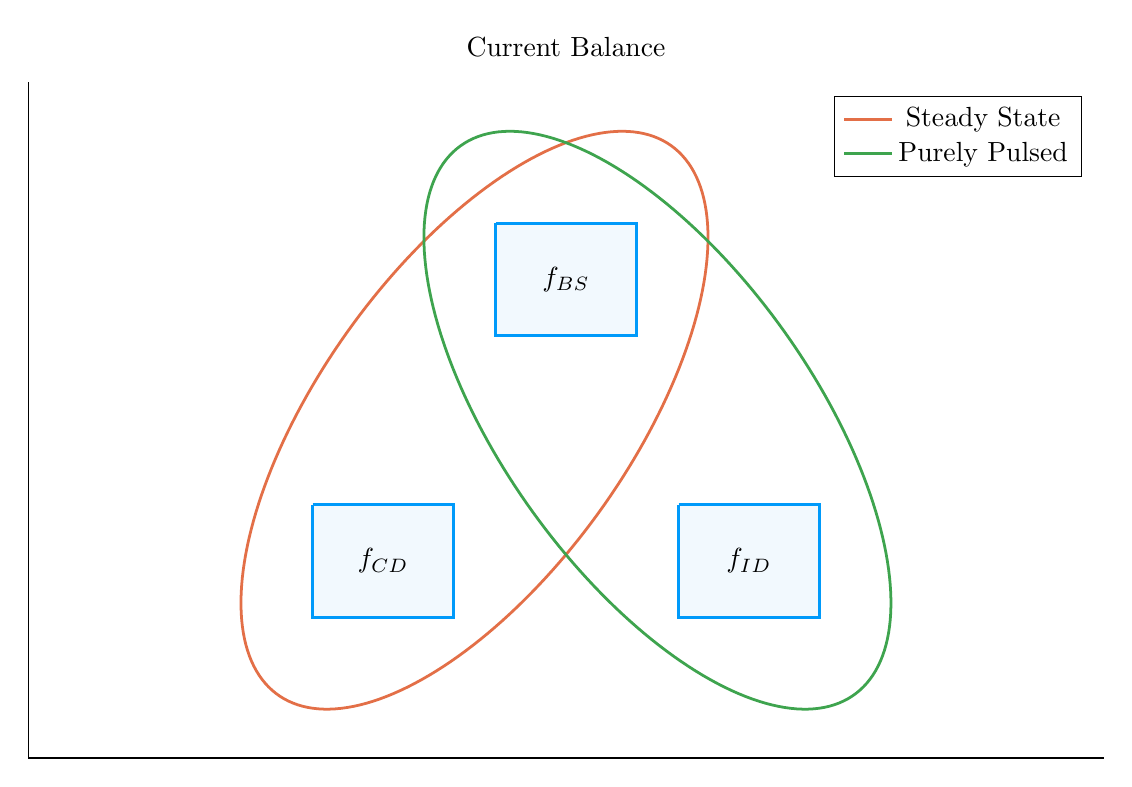
\begin{tikzpicture}[]
\begin{axis}[height = {101.6mm}, axis equal = {true}, ylabel = {}, title = {Current Balance}, xmin = {-5.773116112756781}, xmax = {5.773116112756781}, ymax = {6}, xlabel = {}, {unbounded coords=jump, scaled x ticks = false, xticklabel style={rotate = 0}, xmajorticks=false, xmajorgrids = false, axis lines* = left, scaled y ticks = false, yticklabel style={rotate = 0}, ymajorticks=false, ymajorgrids = false, axis lines* = left,     xshift = 0.0mm,
    yshift = 0.0mm,
    axis background/.style={fill={rgb,1:red,1.00000000;green,1.00000000;blue,1.00000000}}
}, ymin = {-6}, width = {152.4mm}]\addplot+ [color = {rgb,1:red,0.00000000;green,0.60560316;blue,0.97868012},
draw opacity=1.0,
line width=1,
solid,mark = none,
mark size = 2.0,
mark options = {
    color = {rgb,1:red,0.00000000;green,0.00000000;blue,0.00000000}, draw opacity = 1.0,
    fill = {rgb,1:red,0.00000000;green,0.60560316;blue,0.97868012}, fill opacity = 1.0,
    line width = 1,
    rotate = 0,
    solid
},fill = {rgb,1:red,0.00000000;green,0.60560316;blue,0.97868012}, fill opacity=0.05,forget plot]coordinates {
(-1.25, 3.5)
(1.25, 3.5)
(1.25, 1.5)
(-1.25, 1.5)
(-1.25, 3.5)
};
\addplot+ [color = {rgb,1:red,0.00000000;green,0.60560316;blue,0.97868012},
draw opacity=1.0,
line width=1,
solid,mark = none,
mark size = 2.0,
mark options = {
    color = {rgb,1:red,0.00000000;green,0.00000000;blue,0.00000000}, draw opacity = 1.0,
    fill = {rgb,1:red,0.00000000;green,0.60560316;blue,0.97868012}, fill opacity = 1.0,
    line width = 1,
    rotate = 0,
    solid
},fill = {rgb,1:red,0.00000000;green,0.60560316;blue,0.97868012}, fill opacity=0.05,forget plot]coordinates {
(-4.5, -1.5)
(-2.0, -1.5)
(-2.0, -3.5)
(-4.5, -3.5)
(-4.5, -1.5)
};
\addplot+ [color = {rgb,1:red,0.00000000;green,0.60560316;blue,0.97868012},
draw opacity=1.0,
line width=1,
solid,mark = none,
mark size = 2.0,
mark options = {
    color = {rgb,1:red,0.00000000;green,0.00000000;blue,0.00000000}, draw opacity = 1.0,
    fill = {rgb,1:red,0.00000000;green,0.60560316;blue,0.97868012}, fill opacity = 1.0,
    line width = 1,
    rotate = 0,
    solid
},fill = {rgb,1:red,0.00000000;green,0.60560316;blue,0.97868012}, fill opacity=0.05,forget plot]coordinates {
(2.0, -1.5)
(4.5, -1.5)
(4.5, -3.5)
(2.0, -3.5)
(2.0, -1.5)
};
\addplot+ [color = {rgb,1:red,0.88887350;green,0.43564919;blue,0.27812294},
draw opacity=1.0,
line width=1,
solid,mark = none,
mark size = 2.0,
mark options = {
    color = {rgb,1:red,0.00000000;green,0.00000000;blue,0.00000000}, draw opacity = 1.0,
    fill = {rgb,1:red,0.88887350;green,0.43564919;blue,0.27812294}, fill opacity = 1.0,
    line width = 1,
    rotate = 0,
    solid
}]coordinates {
(1.8698661812068136, 4.877080107549691)
(1.7975582266118808, 4.9252162522328415)
(1.7218385915440537, 4.9684428342438745)
(1.6427827549822935, 5.006716764385765)
(1.5604695215037632, 5.03999989037258)
(1.4749809427297138, 5.068259034860505)
(1.3864022355346433, 5.091466028519745)
(1.2948216971002622, 5.109597738114323)
(1.2003306168989445, 5.122636089561793)
(1.1030231856943935, 5.130568085949879)
(1.0029964016502424, 5.133385820492077)
(0.9003499736401737, 5.131086484409318)
(0.7951862218559462, 5.123672369729815)
(0.6876099758124048, 5.111150867004319)
(0.5777284698511354, 5.093534457939059)
(0.46565123624694493, 5.07084070295371)
(0.35148999602370634, 5.043092223676775)
(0.23535854758841435, 5.010316680395862)
(0.11737265329445545, 4.972546744485303)
(-0.00235007595282255, 4.929820065838624)
(-0.12369029793321751, 4.882179235338303)
(-0.2465270580745944, 4.829671742400261)
(-0.37073791002303214, 4.77234992763537)
(-0.49619903770001583, 4.710270930675205)
(-0.6227853787249911, 4.643496633214007)
(-0.7503707490802689, 4.572093597323671)
(-0.878827968893996, 4.496132999103221)
(-1.0080289892158198, 4.415690557728926)
(-1.137845019658864, 4.330846459975782)
(-1.26814665678079, 4.241685280285592)
(-1.3988040130759585, 4.148295896461316)
(-1.5296868464501256, 4.050771401071749)
(-1.6606646900485882, 3.949209008654826)
(-1.7916069823083864, 3.8437099588120507)
(-1.9223831971049103, 3.734379415290662)
(-2.0528629738631725, 3.6213263611541278)
(-2.1829162475040724, 3.5046634901454468)
(-2.3124133780960925, 3.3845070943515854)
(-2.4412252800831986, 3.26097694828099)
(-2.5692235509601344, 3.1341961894697543)
(-2.696280599266827, 3.004291195735447)
(-2.822269771774333, 2.8713914592009493)
(-2.947065479735527, 2.735629457213896)
(-3.0705433240746993, 2.597140520290374)
(-3.192580219391261, 2.4560626972145165)
(-3.3130545166539442, 2.3125366174284774)
(-3.4318461244632026, 2.166705350849943)
(-3.5488366287609345, 2.0187142652569277)
(-3.6639094108681878, 1.8687108813820061)
(-3.776949763733194, 1.7168447258604496)
(-3.8878450062738565, 1.5632671821788118)
(-3.9964845957006974, 1.4081313397725874)
(-4.1027602377083205, 1.2515918414233274)
(-4.206565994425528, 1.0938047291073505)
(-4.307798390016492, 0.9349272884497156)
(-4.4063565138277205, 0.7751178919384804)
(-4.502142120977991, 0.614535841055565)
(-4.595059730290983, 0.4533412074815748)
(-4.685016719472996, 0.29169467353285894)
(-4.771923417440856, 0.12975737198989234)
(-4.8556931937080146, -0.032309274523392384)
(-4.936242544739693, -0.1943437144491822)
(-5.013491177191022, -0.3561844283338884)
(-5.087362087945198, -0.5176700898342566)
(-5.157781640871865, -0.6786397265309694)
(-5.224679640229201, -0.8389328803894542)
(-5.287989400636577, -0.9983897677079463)
(-5.347647813547976, -1.1568514383933535)
(-5.403595410159981, -1.3141599344061687)
(-5.455776420691558, -1.4701584472164726)
(-5.504138829976595, -1.6246914741140965)
(-5.548634429313749, -1.7776049732170973)
(-5.589218864521925, -1.9287465170240605)
(-5.625851680153492, -2.0779654443571474)
(-5.658496359821148, -2.225113010544426)
(-5.687120362598258, -2.3700425356918093)
(-5.711695155456349, -2.5126095508967543)
(-5.732196241707455, -2.6526719422580065)
(-5.74860318542295, -2.7900900925378296)
(-5.760899631804527, -2.9247270203354994)
(-5.769073323487013, -3.0564485166333526)
(-5.773116112756781, -3.1851232785792454)
(-5.773023969673565, -3.3106230403720964)
(-5.768796986087595, -3.432822701120024)
(-5.760439375548035, -3.551600449543642)
(-5.747959469102832, -3.6668378854001826)
(-5.731369706994138, -3.778420137507439)
(-5.710686626257609, -3.8862359782498594)
(-5.685930844237935, -3.9901779344526522)
(-5.657127038037011, -4.090142394513381)
(-5.624303919915274, -4.186029711684261)
(-5.587494208670695, -4.2777443034022165)
(-5.546734597023965, -4.365194746567642)
(-5.502065715042401, -4.448293868676952)
(-5.453532089639006, -4.526958834718015)
(-5.4011821001870715, -4.601111229741906)
(-5.345067930294576, -4.67067713702862)
(-5.285245515786418, -4.735587211768881)
(-5.221774488946376, -4.795776750188546)
(-5.154718119074351, -4.851185754046737)
(-5.084143249418149, -4.901758990443393)
(-5.010120230542682, -4.947446046876624)
(-4.932722850202994, -4.98820138149499)
(-4.852028259791015, -5.023984368494613)
(-4.768116897429388, -5.054759338615853)
(-4.681072407788987, -5.080495614699213)
(-4.590981558710103, -5.101167542264987)
(-4.497934154710361, -5.116754515086211)
(-4.40202294746563, -5.127240995729401)
(-4.303343543353135, -5.132616531042591)
(-4.201994308148942, -5.132875762575277)
(-4.098076268974807, -5.1280184319198305)
(-3.9916930135921564, -5.118049380969083)
(-3.88295058714354, -5.102978547089826)
(-3.7719573864445346, -5.082820953217027)
(-3.658824051931438, -5.0575966928786364)
(-3.543663357372476, -5.02733091016593)
(-3.4265900974524626, -4.9920537746693245)
(-3.3077209733429527, -4.951800451404678)
(-3.1871744763719843, -4.906611065760036)
(-3.065070769909341, -4.8565306634977725)
(-2.941531569585093, -4.801609165851993)
(-2.816680021960811, -4.741901319765965)
(-2.690640581774395, -4.677466643319172)
(-2.5635388878808865, -4.608369366398399)
(-2.435501638012921, -4.5346783666719865)
(-2.306656462485676, -4.456467100931064)
(-2.1771317969721977, -4.373813531866238)
(-2.047056754475925, -4.286800050352669)
(-1.9165609966280504, -4.1955133933210735)
(-1.785774604437966, -4.100044557296444)
(-1.654827948625708, -4.00048870769076)
(-1.523851559665576, -3.896945083940012)
(-1.3929759976705065, -3.7895169005801836)
(-1.26233172224694, -3.678311244360763)
(-1.132048962449818, -3.5634389674983264)
(-1.0022575869674537, -3.4450145771766545)
(-0.8730869746655892, -3.323156121403477)
(-0.7446658856197179, -3.1979850713376368)
(-0.6171223327642645, -3.069626200204022)
(-0.49058345428648176, -2.938207458916877)
(-0.3651753868923626, -2.803859848535569)
(-0.24102314007082093, -2.666717289679875)
(-0.11825047148150092, -2.526916489034983)
(0.0030202364095237577, -2.384596803079324)
(0.12266809832327996, -2.2399000991709683)
(0.2405738466689491, -2.09297061413119)
(0.3566199504324037, -1.9439548104660527)
(0.4706907323336891, -1.7930012303693847)
(0.5826724841366269, -1.6402603476527216)
(0.6924535799956866, -1.4858844177497015)
(0.7999245877270309, -1.3300273259445707)
(0.9049783778929097, -1.1728444339759707)
(1.0075102305906167, -1.0144924251689658)
(1.1074179398395505, -0.8551291482497284)
(1.20460191546238, -0.6949134599984598)
(1.2989652823586764, -0.534005066897528)
(1.3904139770721349, -0.3725643659325606)
(1.478856841555075, -0.210752284705227)
(1.564205714036751, -0.04873012101713625)
(1.6463755169049392, 0.11334061791535466)
(1.725284341513138, 0.27529837645501054)
(1.8008535298288972, 0.4369817115859278)
(1.8730077528418523, 0.598229453843409)
(1.9416750856533156, 0.7588808679712085)
(2.0067870791725912, 0.9187758131459416)
(2.0682788283485025, 1.0777549026089095)
(2.126089036868173, 1.2356596625463219)
(2.1801600782585133, 1.3923326900594108)
(2.2304380533295443, 1.5476178100670777)
(2.2768728439022907, 1.7013602309846187)
(2.3194181627676604, 1.8534066990233193)
(2.358031599826549, 2.0036056509571933)
(2.392674664365143, 2.1518073652044736)
(2.423312823423304, 2.2978641110733555)
(2.4499155362177776, 2.4416302960231726)
(2.4724562845859026, 2.5829626107941834)
(2.490912599419497, 2.7217201722613846)
(2.505266083062553, 2.857764663869852)
(2.5155024276504205, 2.990960473511697)
(2.521611429372199, 3.12117482870718)
(2.5235869986421147, 3.2482779289551793)
(2.5214271661697554, 3.3721430751211794)
(2.515134084923101, 3.4926467957337035)
(2.5047140279823985, 3.609668970063368)
(2.4901773822870172, 3.7230929478618506)
(2.471538638281525, 3.8328056656413696)
(2.448816375471295, 3.9386977593788552)
(2.422033243902053, 4.040663673532358)
(2.391215941581816, 4.1386017662611385)
(2.356395187867742, 4.232414410744436)
(2.317605692844403, 4.322008092498024)
(2.274886122724018, 4.4072935025914814)
(2.2282790613031342, 4.488185626673267)
(2.1778309675141685, 4.564603829714885)
(2.123592129114139, 4.636471936389625)
(2.06561661255673, 4.70371830700579)
(2.0039622090976756, 4.766275908918702)
(1.9386903771871857, 4.824082383350291)
(1.869866181206814, 4.877080107549691)
};
\addlegendentry{Steady State}
\addplot+ [color = {rgb,1:red,0.24222430;green,0.64327509;blue,0.30444865},
draw opacity=1.0,
line width=1,
solid,mark = none,
mark size = 2.0,
mark options = {
    color = {rgb,1:red,0.00000000;green,0.00000000;blue,0.00000000}, draw opacity = 1.0,
    fill = {rgb,1:red,0.24222430;green,0.64327509;blue,0.30444865}, fill opacity = 1.0,
    line width = 1,
    rotate = 0,
    solid
}]coordinates {
(-1.8698661812068136, 4.877080107549691)
(-1.7975582266118808, 4.9252162522328415)
(-1.7218385915440537, 4.9684428342438745)
(-1.6427827549822935, 5.006716764385765)
(-1.5604695215037632, 5.03999989037258)
(-1.4749809427297138, 5.068259034860505)
(-1.3864022355346433, 5.091466028519745)
(-1.2948216971002622, 5.109597738114323)
(-1.2003306168989445, 5.122636089561793)
(-1.1030231856943935, 5.130568085949879)
(-1.0029964016502424, 5.133385820492077)
(-0.9003499736401737, 5.131086484409318)
(-0.7951862218559462, 5.123672369729815)
(-0.6876099758124048, 5.111150867004319)
(-0.5777284698511354, 5.093534457939059)
(-0.46565123624694493, 5.07084070295371)
(-0.35148999602370634, 5.043092223676775)
(-0.23535854758841435, 5.010316680395862)
(-0.11737265329445545, 4.972546744485303)
(0.00235007595282255, 4.929820065838624)
(0.12369029793321751, 4.882179235338303)
(0.2465270580745944, 4.829671742400261)
(0.37073791002303214, 4.77234992763537)
(0.49619903770001583, 4.710270930675205)
(0.6227853787249911, 4.643496633214007)
(0.7503707490802689, 4.572093597323671)
(0.878827968893996, 4.496132999103221)
(1.0080289892158198, 4.415690557728926)
(1.137845019658864, 4.330846459975782)
(1.26814665678079, 4.241685280285592)
(1.3988040130759585, 4.148295896461316)
(1.5296868464501256, 4.050771401071749)
(1.6606646900485882, 3.949209008654826)
(1.7916069823083864, 3.8437099588120507)
(1.9223831971049103, 3.734379415290662)
(2.0528629738631725, 3.6213263611541278)
(2.1829162475040724, 3.5046634901454468)
(2.3124133780960925, 3.3845070943515854)
(2.4412252800831986, 3.26097694828099)
(2.5692235509601344, 3.1341961894697543)
(2.696280599266827, 3.004291195735447)
(2.822269771774333, 2.8713914592009493)
(2.947065479735527, 2.735629457213896)
(3.0705433240746993, 2.597140520290374)
(3.192580219391261, 2.4560626972145165)
(3.3130545166539442, 2.3125366174284774)
(3.4318461244632026, 2.166705350849943)
(3.5488366287609345, 2.0187142652569277)
(3.6639094108681878, 1.8687108813820061)
(3.776949763733194, 1.7168447258604496)
(3.8878450062738565, 1.5632671821788118)
(3.9964845957006974, 1.4081313397725874)
(4.1027602377083205, 1.2515918414233274)
(4.206565994425528, 1.0938047291073505)
(4.307798390016492, 0.9349272884497156)
(4.4063565138277205, 0.7751178919384804)
(4.502142120977991, 0.614535841055565)
(4.595059730290983, 0.4533412074815748)
(4.685016719472996, 0.29169467353285894)
(4.771923417440856, 0.12975737198989234)
(4.8556931937080146, -0.032309274523392384)
(4.936242544739693, -0.1943437144491822)
(5.013491177191022, -0.3561844283338884)
(5.087362087945198, -0.5176700898342566)
(5.157781640871865, -0.6786397265309694)
(5.224679640229201, -0.8389328803894542)
(5.287989400636577, -0.9983897677079463)
(5.347647813547976, -1.1568514383933535)
(5.403595410159981, -1.3141599344061687)
(5.455776420691558, -1.4701584472164726)
(5.504138829976595, -1.6246914741140965)
(5.548634429313749, -1.7776049732170973)
(5.589218864521925, -1.9287465170240605)
(5.625851680153492, -2.0779654443571474)
(5.658496359821148, -2.225113010544426)
(5.687120362598258, -2.3700425356918093)
(5.711695155456349, -2.5126095508967543)
(5.732196241707455, -2.6526719422580065)
(5.74860318542295, -2.7900900925378296)
(5.760899631804527, -2.9247270203354994)
(5.769073323487013, -3.0564485166333526)
(5.773116112756781, -3.1851232785792454)
(5.773023969673565, -3.3106230403720964)
(5.768796986087595, -3.432822701120024)
(5.760439375548035, -3.551600449543642)
(5.747959469102832, -3.6668378854001826)
(5.731369706994138, -3.778420137507439)
(5.710686626257609, -3.8862359782498594)
(5.685930844237935, -3.9901779344526522)
(5.657127038037011, -4.090142394513381)
(5.624303919915274, -4.186029711684261)
(5.587494208670695, -4.2777443034022165)
(5.546734597023965, -4.365194746567642)
(5.502065715042401, -4.448293868676952)
(5.453532089639006, -4.526958834718015)
(5.4011821001870715, -4.601111229741906)
(5.345067930294576, -4.67067713702862)
(5.285245515786418, -4.735587211768881)
(5.221774488946376, -4.795776750188546)
(5.154718119074351, -4.851185754046737)
(5.084143249418149, -4.901758990443393)
(5.010120230542682, -4.947446046876624)
(4.932722850202994, -4.98820138149499)
(4.852028259791015, -5.023984368494613)
(4.768116897429388, -5.054759338615853)
(4.681072407788987, -5.080495614699213)
(4.590981558710103, -5.101167542264987)
(4.497934154710361, -5.116754515086211)
(4.40202294746563, -5.127240995729401)
(4.303343543353135, -5.132616531042591)
(4.201994308148942, -5.132875762575277)
(4.098076268974807, -5.1280184319198305)
(3.9916930135921564, -5.118049380969083)
(3.88295058714354, -5.102978547089826)
(3.7719573864445346, -5.082820953217027)
(3.658824051931438, -5.0575966928786364)
(3.543663357372476, -5.02733091016593)
(3.4265900974524626, -4.9920537746693245)
(3.3077209733429527, -4.951800451404678)
(3.1871744763719843, -4.906611065760036)
(3.065070769909341, -4.8565306634977725)
(2.941531569585093, -4.801609165851993)
(2.816680021960811, -4.741901319765965)
(2.690640581774395, -4.677466643319172)
(2.5635388878808865, -4.608369366398399)
(2.435501638012921, -4.5346783666719865)
(2.306656462485676, -4.456467100931064)
(2.1771317969721977, -4.373813531866238)
(2.047056754475925, -4.286800050352669)
(1.9165609966280504, -4.1955133933210735)
(1.785774604437966, -4.100044557296444)
(1.654827948625708, -4.00048870769076)
(1.523851559665576, -3.896945083940012)
(1.3929759976705065, -3.7895169005801836)
(1.26233172224694, -3.678311244360763)
(1.132048962449818, -3.5634389674983264)
(1.0022575869674537, -3.4450145771766545)
(0.8730869746655892, -3.323156121403477)
(0.7446658856197179, -3.1979850713376368)
(0.6171223327642645, -3.069626200204022)
(0.49058345428648176, -2.938207458916877)
(0.3651753868923626, -2.803859848535569)
(0.24102314007082093, -2.666717289679875)
(0.11825047148150092, -2.526916489034983)
(-0.0030202364095237577, -2.384596803079324)
(-0.12266809832327996, -2.2399000991709683)
(-0.2405738466689491, -2.09297061413119)
(-0.3566199504324037, -1.9439548104660527)
(-0.4706907323336891, -1.7930012303693847)
(-0.5826724841366269, -1.6402603476527216)
(-0.6924535799956866, -1.4858844177497015)
(-0.7999245877270309, -1.3300273259445707)
(-0.9049783778929097, -1.1728444339759707)
(-1.0075102305906167, -1.0144924251689658)
(-1.1074179398395505, -0.8551291482497284)
(-1.20460191546238, -0.6949134599984598)
(-1.2989652823586764, -0.534005066897528)
(-1.3904139770721349, -0.3725643659325606)
(-1.478856841555075, -0.210752284705227)
(-1.564205714036751, -0.04873012101713625)
(-1.6463755169049392, 0.11334061791535466)
(-1.725284341513138, 0.27529837645501054)
(-1.8008535298288972, 0.4369817115859278)
(-1.8730077528418523, 0.598229453843409)
(-1.9416750856533156, 0.7588808679712085)
(-2.0067870791725912, 0.9187758131459416)
(-2.0682788283485025, 1.0777549026089095)
(-2.126089036868173, 1.2356596625463219)
(-2.1801600782585133, 1.3923326900594108)
(-2.2304380533295443, 1.5476178100670777)
(-2.2768728439022907, 1.7013602309846187)
(-2.3194181627676604, 1.8534066990233193)
(-2.358031599826549, 2.0036056509571933)
(-2.392674664365143, 2.1518073652044736)
(-2.423312823423304, 2.2978641110733555)
(-2.4499155362177776, 2.4416302960231726)
(-2.4724562845859026, 2.5829626107941834)
(-2.490912599419497, 2.7217201722613846)
(-2.505266083062553, 2.857764663869852)
(-2.5155024276504205, 2.990960473511697)
(-2.521611429372199, 3.12117482870718)
(-2.5235869986421147, 3.2482779289551793)
(-2.5214271661697554, 3.3721430751211794)
(-2.515134084923101, 3.4926467957337035)
(-2.5047140279823985, 3.609668970063368)
(-2.4901773822870172, 3.7230929478618506)
(-2.471538638281525, 3.8328056656413696)
(-2.448816375471295, 3.9386977593788552)
(-2.422033243902053, 4.040663673532358)
(-2.391215941581816, 4.1386017662611385)
(-2.356395187867742, 4.232414410744436)
(-2.317605692844403, 4.322008092498024)
(-2.274886122724018, 4.4072935025914814)
(-2.2282790613031342, 4.488185626673267)
(-2.1778309675141685, 4.564603829714885)
(-2.123592129114139, 4.636471936389625)
(-2.06561661255673, 4.70371830700579)
(-2.0039622090976756, 4.766275908918702)
(-1.9386903771871857, 4.824082383350291)
(-1.869866181206814, 4.877080107549691)
};
\addlegendentry{Purely Pulsed}
\node at (axis cs:0, 2.5) [,
color={rgb,1:red,0.00000000;green,0.00000000;blue,0.00000000}, draw opacity=1.0,
rotate=0.0
] {$f_{BS}$};
\node at (axis cs:-3.25, -2.5) [,
color={rgb,1:red,0.00000000;green,0.00000000;blue,0.00000000}, draw opacity=1.0,
rotate=0.0
] {$f_{CD}$};
\node at (axis cs:3.25, -2.5) [,
color={rgb,1:red,0.00000000;green,0.00000000;blue,0.00000000}, draw opacity=1.0,
rotate=0.0
] {$f_{ID}$};
\end{axis}

\end{tikzpicture}

	\end{adjustbox}
%	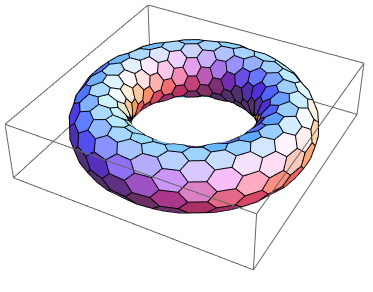
\includegraphics[width=0.75\textwidth]{images/test_image}
	\caption{Current Balance in a Tokamak} ~\\
	\small In a tokamak, there needs to be a certain amount of current -- and that current has to come from somewhere. All good reactors have an adequate bootstrap current. What provides the remaining current is what distinguishes steady state from pulsed operation.
\end{figure}

The arguments against this are mainly technical: why build two difficult auxiliary systems when one is needed -- especially when they probably work against each other. Although rational, \replaced{it may turn out that the larger current achievable with two sources leads to a smaller, more economic machine.}{the argument implicitly assumes a current is achievable through only one source (i.e.\ either through LHCD or from a central solenoid). Using two may allow for stronger plasma currents.}

\section{Bridging Confinement Scalings -- Daedalus}

The final potential reactor -- Daedalus -- is designed \replaced{so that it can be}{to collect as many scaling laws as possible. As a baseline, it should be able to} run in H-Mode, L-Mode, and I-Mode. Because L-Mode is available on any machine, the first step is \added{actually} building under H-Mode. The goal then is to find reactors that can also reach I-Mode -- \replaced{simultaneously}{thus} improving the scaling law's fit and \added{possibly} making the actual reactor more \replaced{economic}{cost effective}.

Presented below are the three confinement scaling laws, as well as the generalized formula. As should be noted, the I-Mode scaling currently lacks a true radial dependence -- as it has only been found on two machines. This is one reason Daedalus would be so valuable.

\begin{equation}
  \tau_E^G = K_\tau \, H \, \frac{
    I_P^{\,\alpha_I} \, R_0^{\,\alpha_R} \, a^{\,\alpha_a} \, \kappa^{\,\alpha_\kappa} \ \overline{n}^{\,\alpha_n} \, B_0^{\,\alpha_B} \, A^{\,\alpha_A}
  }{ P_{src} ^ {\,\alpha_P} }
  \tag{\ref{eq:tau_gen}}
\end{equation}

\begin{equation}
  \tau_E^H = 0.145 \, H \, \frac{
    I_P^{0.93} \, R_0^{1.39} \, a^{0.58} \, \kappa^{0.78} \ \overline{n}^{\, 0.41} \, B_0^{0.15} \, A^{0.19}
  }{ P_{src} ^ {\,0.69} }
  \tag{\ref{eq:tau_h}}
\end{equation}
\begin{equation}
  \tau_E^L = 0.048\, H \, \frac{
    I_P^{0.85} \, R_0^{1.2} \, a^{0.3} \, \kappa^{0.5} \ \overline{n}^{\, 0.1} \, B_0^{0.2} \, A^{0.5} }{ P_{src} ^ {\,0.5} }
\end{equation}
\begin{equation}
  \tau_E^I = \frac{ 0.014 \, H }{ 0.68 ^ {\lambda_R} \cdot 0.22 ^ {\lambda_a} } \cdot \frac{ I_P^{0.69} \, R_0^{\lambda_R} \, a^{\lambda_a} \, \kappa^{0.0} \ \overline{n}^{\, 0.17} \, B_0^{0.77} \, A^{0.0} }{ P_{src} ^ {\,0.29} }
\end{equation}
\begin{equation}
	\lambda_R + \lambda_a = 2.2
\end{equation}

A final point to make is reemphasizing that the I-Mode scaling law is \replaced{significantly underdeveloped}{not battle-tested.} It is the target of ongoing research at the MIT PSFC.

\section{Addressing Model Shortcomings}

Before moving on to the final conclusions, we will give a quick recap of \replaced{several of the more overly simplified phenomena in}{the more audacious simplifications used within} this fusion systems framework. These include: approximating temperature profiles as simple parabolas, neglecting all radiation except Bremsstrahlung, and handling flux sources at too basic a level. \added{This list is non-comprehensive, as more sophisticated analysis would also help: the divertor heat load, the neutron wall loading, etc.}

\subsection{Integrating Pedestal Temperature Profiles}

\replaced{One of the biggest shortcomings of this model is not handling plasma profiles self-consistently -- instead replacing them with simple parabolas.}{The most dubious simplification in the code at this point is modeling temperature profiles as parabolas.} Although these parabolas work for densities and L-Mode plasma temperatures, the same cannot be said about H-Mode temperatures. This is because they have a distinct pedestal region on the outer edge of the plasma.

The usage of pedestal temperatures -- discussed in the appendix -- improves two aspects of the model: the fusion power and the bootstrap current. These were shown in the results to be over-calculated and underestimated, respectively. Pedestals, having a lower core temperature, would decrease the total fusion power. As well, they would boost bootstrap current due to the quick drop near the plasma's edge (i.e.\ they have a large derivative there). 

These improvements could easily be added to the code, because temperature was addressed as a difficult parameter to handle from the beginning.

\subsection{Expanding the Radiation Loss Term}

The next area that would be improved by more sophisticated theory would be the radiation loss term. From before, it was pointed out that the Bremsstrahlung radiation was the dominant term within the plasma core and, therefore, provided a first-order approximation. Drawing the radiation losses closer to real world values would involve adding line radiation and synchrotron radiation. The former of which would be needed as high-Z impurities become more important.

\subsection{Taking Flux Sources Seriously}

The final oversimplification in the model deals with the flux sources involved in a pulsed reactor -- existing at almost every level. First, the derivation of flux balance started with a simple transformer between a solenoid primary and a plasma secondary. \deleted{Even this initial step is probably too simple.}

After we developed an equation for flux balance, we compared it to ones in the literature (i.e.\ PROCESS) to build confidence in the model. To draw this equation closer to theirs, we then added a PF coil contribution a posteriori. This implicitly ignored coupling between most of the components. Thus leading to another source of error for the model. Moreover, this formula for PF coil contribution was much simpler than ones found in other fusion systems codes.

Even though this model may be extremely simple, it does remarkably well at matching more sophisticated codes -- and does so at a much faster pace. These suggestions were \deleted{all} just ways to \replaced{account for more realistic physics.}{draw results closer to real world values.}

%\end{document}
